\documentclass[varwidth, border=10pt]{standalone}
\usepackage{tikz}
\usepackage[]{xcolor}
\usepackage{subcaption}
\usepackage{tikz}

% % \usetikzlibrary{positioning}
% \usetikzlibrary{arrows,backgrounds}
% 
% \usepackage{amsmath, amsthm, amssymb}
% \input{commondefinitions}
% 	
% 
% 
% \begin{document}
% \pagestyle{empty}
% %\providecommand{\openone}{\leavevmode\hbox{\small1\kern-3.8pt\normalsize1}}
% 
% % \documentclass[12pt]{article}
% % \usepackage{psfrag}
% \usepackage{tikz}
% % \usetikzlibrary{positioning}
% % \usetikzlibrary{arrows,backgrounds}
 \usetikzlibrary{calc}
\usepackage{bbold}

\usepackage{tikz}
\usetikzlibrary{arrows}
\usetikzlibrary{quantikz}


\usepackage{amsmath, amsthm, amssymb}
\colorlet{coscolor}{blue}

\newcommand{\red}{\color{red}}
\newcommand{\blue}{\color{blue}}
%Colors

\definecolor{max}{rgb}{1,0.54,0.1}
\definecolor{medium}{rgb}{1,0.8,0.6}
\definecolor{min}{rgb}{1,0.9,0.8}
\begin{document}
\thispagestyle{empty}


\begin{tikzpicture}
\node[inner sep=0pt] (curvas) at (0,0)
	{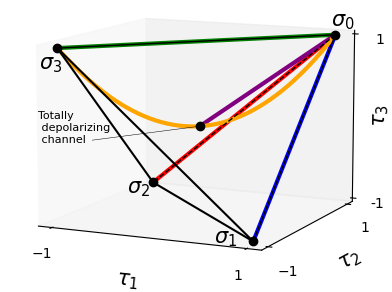
\includegraphics[width=.45\textwidth]{curvas.png}};
\node[inner sep=0pt] (curvas-azar) at (6,0)
	{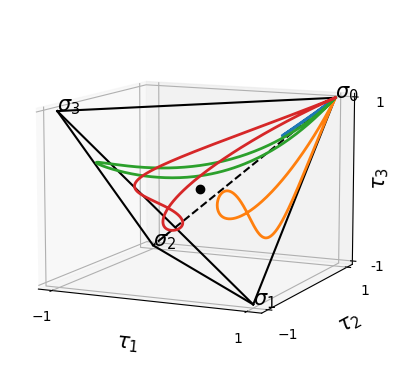
\includegraphics[width=.45\textwidth]{curvas-azar.png}};
\node at (-2,1.95) {(a)};
\node at (4,1.95) {(b)};
\end{tikzpicture}

\end{document}



